\documentclass[a4paper,12pt]{article}
\addtolength{\oddsidemargin}{-1.cm}
\addtolength{\textwidth}{2cm}
\addtolength{\topmargin}{-2cm}
\addtolength{\textheight}{3.5cm}
\newcommand{\HRule}{\rule{\linewidth}{0.5mm}}
\makeindex

\usepackage{titlesec}
\usepackage{longtable}
\usepackage[pdftex]{graphicx}
\usepackage{makeidx}
\usepackage{hyperref}
\usepackage{verbatim}
\hypersetup{
    colorlinks=true,
    linkcolor=blue,
    filecolor=magenta,      
    urlcolor=cyan,
}


% define the title
\author{IMAPKD}
\title{ Testing}
\begin{document}
\setlength{\parskip}{6pt}

% generates the title
\begin{titlepage}

\begin{center}
% Upper part of the page       

\includegraphics[width=1\textwidth]{./University_of_Pretoria_Logo.PNG}\\[0.4cm]  

%Title

\HRule \\[0.4cm]
{\LARGE IMPAKD}\\[0.8cm]
{\LARGE Project $\>$ $\>$   COS 301 Main Project}\\[0.5cm]
{\LARGE Product $\>$ $\>$  Test Plan and Report}\\[0.8cm]
{\LARGE Version $\>$ $\>$  1.2}\\
\HRule \\[4cm]  

% Group Members 

%\begin{minipage}{0.4\textwidth}
%\begin{flushleft} \large

%\emph{\Large Group Members:}\\[0.4cm]    
%\emph{}\\
%{\Large Diana {Obo}} \\
%\emph{}\\
%\emph{}\\
%{\Large Priscilla {Madigoe}}\\
%\emph{}\\
%\emph{}\\
%{\Large Kudzai {Muranga}} \\
%\emph{}\\
%\emph{}\\
%{\Large Sandile {Khumalo}}\\
%\emph{}\\
%\emph{}\\

%\end{flushleft}
%\end{minipage}
%\begin{minipage}{0.4\textwidth}
%\begin{flushright} \large

%\emph{ \Large Student numbers:} \\[0.4cm]  
%\emph{}\\
%{\Large u13134885}\\
%\emph{}\\
%\emph{}\\
%{\Large u13049128}\\
%\emph{}\\
%\emph{}\\
%{\Large u13278012}\\
%\emph{}\\
%\emph{}\\
%{\Large u12031748}\\
%\emph{}\\
%\emph{}\\

%\end{flushright}
%\end{minipage}

{ \huge \bfseries Unit Test Plan and Report}\\[4cm]

% bottom right section of title page

\hfill{\large Prepared by:}\\[0.5cm]
\hfill{\large Member 1- 12031748}\\[0.1cm]
\hfill{\large Member 2- 13278012}\\[0.1cm]
\hfill{\large Member 3- 13134885}\\[0.1cm]
\hfill{\large Member 4- 13049128}\\[0.5cm]
\hfill{\large \today}

\end{center}
\end{titlepage}
\renewcommand{\thesection}{\arabic{section}}

\newpage
\begin{center}
\textsc{\Large IMPAKD link}\\[0.5cm]
For further references see \href{https://github.com/u13278012/IMPAKD/}{gitHub}.
\today
\end{center}
\newpage
\tableofcontents{}

\setcounter{secnumdepth}{4}

\newpage
\section{Introduction}
\subsection{Purpose}
This document combines the unit test plan and report into a single coherent artefact.
Explain the purpose of your system and of this document here. Why is test driven devel-
opment essential to your system.
\subsection{Scope}
The scope of this document is structured as follows. The features that are considered for
testing are listed in section .... Tests that have been identifed from the requirements are
discussed in detail in section .... Furthermore, this document outlines the test environment
and the risks involved in the testing approaches that will be followed. Assumptions and
dependencies of this test plan will also be mentioned. Section 7.1, 7.1 and 9 outlines,
discusses and concludes on the results of the tests, respectively.
\subsection{Test Environment}
\subsection{Assumptions and Dependencies}

%Unit test Plan page
\newpage
\begin{center}
{\huge \bfseries Unit Test Plan}\\[0.5cm]
\end{center}
\section{Test Items}

\section{Functional Features to be Tested}
\begin{center}
 \begin{tabular}{||c| c| c| c||} 
 \hline
 Feature ID & RDS Source & Summary & Test Case ID \\ [0.5ex]
 1 & Implementation.PIO.FrontEnd.app.addProperty & Passed & 01 \\
 2 & Implementation.PIO.BackEnd.test.Test & Passed & 02 \\
 3 & Implementation.PIO.BackEnd.test.Test & Passed & 03 \\
 4 & Implementation.PIO.BackEnd.test.Test & Passed & 04 \\
 5 & Implementation.PIO.BackEnd.test.Test & Passed & 05 \\
 6 & Implementation.PIO.FrontEnd.app.addProperty & Passed & 06 \\



 \hline\hline
 %1 & 6 & 87837 & 787 \\ 
 %\hline
 %2 & 7 & 78 & 5415 \\
 %\hline
 %3 & 545 & 778 & 7507 \\
 %\hline
 %4 & 545 & 18744 & 7560 \\
 %\hline
 %5 & 88 & 788 & 6344 \\ [1ex] 
 %\hline
\end{tabular}
\end{center}

\section{Test Cases}
\subsection{Test Case 1: Test if the encoded string sent to the back-end contains the right information}
\subsubsection{Condition 1: session is created}
\paragraph{Objective:}The purpose of this test is to test if the infomation being passed by the \$http request is correct 
\paragraph{Input:}The following inputs will be used to test this functionality:\\
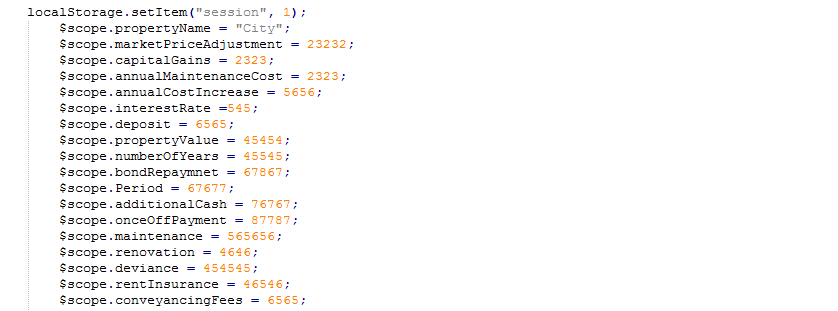
\includegraphics[width=1\textwidth]{./Images/input.png}

\paragraph{Outcome: }The mocked user input will have to match the equivalent encoded string provided in the expected parameter\\
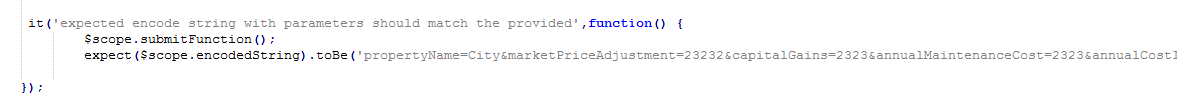
\includegraphics[width=1\textwidth]{./Images/expectedCase1.png}

\subsection{Test Case 2: Retrieve a property and test if the Property name is as expected}
\subsubsection{Condition 1: Back-End Server must be running}
\paragraph{Objective:}The purpose of this test is to test the getProperties function is it returns the correct property
\paragraph{Input:} user profile ID and a property ID , (1 ,8)\\
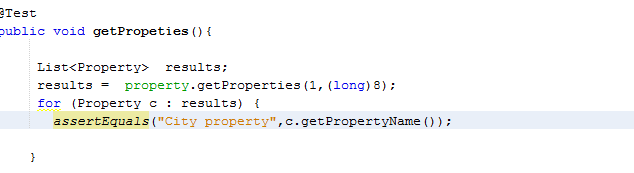
\includegraphics[width=1\textwidth]{./Images/expectedCase2.png}

\paragraph{Outcome: } The function will throw a ArithmeticException

\subsection{Test Case 3: Add a property with negative ID}
\subsubsection{Condition 1: Back-End Server must be running}
\paragraph{Objective:}The purpose of this test is to check how the validation of add property works when invalid values are injected 
\paragraph{Input:} Negative values are used as input , -1\\
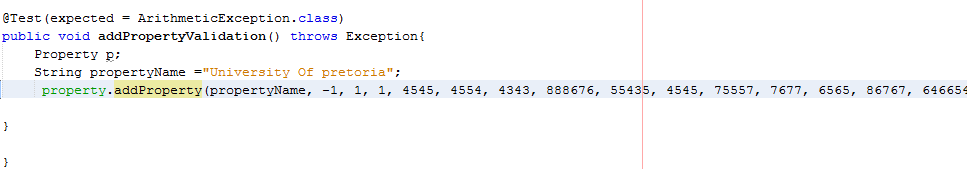
\includegraphics[width=1\textwidth]{./Images/input3.png}

\paragraph{Outcome: } The function will throw a ArithmeticException

\subsection{Test Case 4: Delete a property with an none-existing ID}
\subsubsection{Condition 1: Back-End Server must be running}
\paragraph{Objective:}The purpose of this test is to check how the validation of delete property works when invalid values are injected 
\paragraph{Input:}Nonexisting , negative values such  -1\\
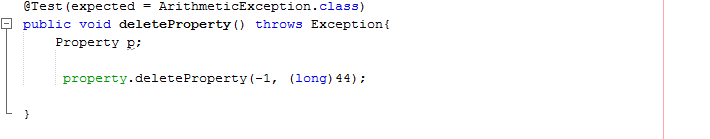
\includegraphics[width=1\textwidth]{./Images/input4.png}

\paragraph{Outcome: } The function will throw a ArithmeticException

\subsection{Test Case 5: Find a property that does not exist}
\subsubsection{Condition 1: Back-End Server must be running}
\paragraph{Objective:}The purpose of this test is to test how the function handles a request when an id of a none-existing property is sent
\paragraph{Input:} Any propertyID Value that is not in the database , 33\\
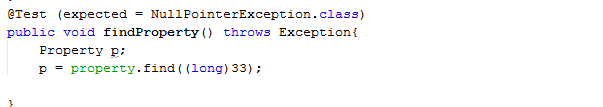
\includegraphics[width=1\textwidth]{./Images/input5.png}

\paragraph{Outcome: } The function will throw a NullPointerException

\subsection{Test Case 6: Set AddedProperty boolean to true if property has been inserted}
\subsubsection{Condition 1: Back-End Server must be running}
\paragraph{Objective:}The purpose of this function is to test in the front-end application whether the property was successful sent to the back-end and persisted in the database, the \$http request's success function initialises the boolean to true if it was successful otherwise it is initialised to false by the error function
\paragraph{Input:} endcoded String\\
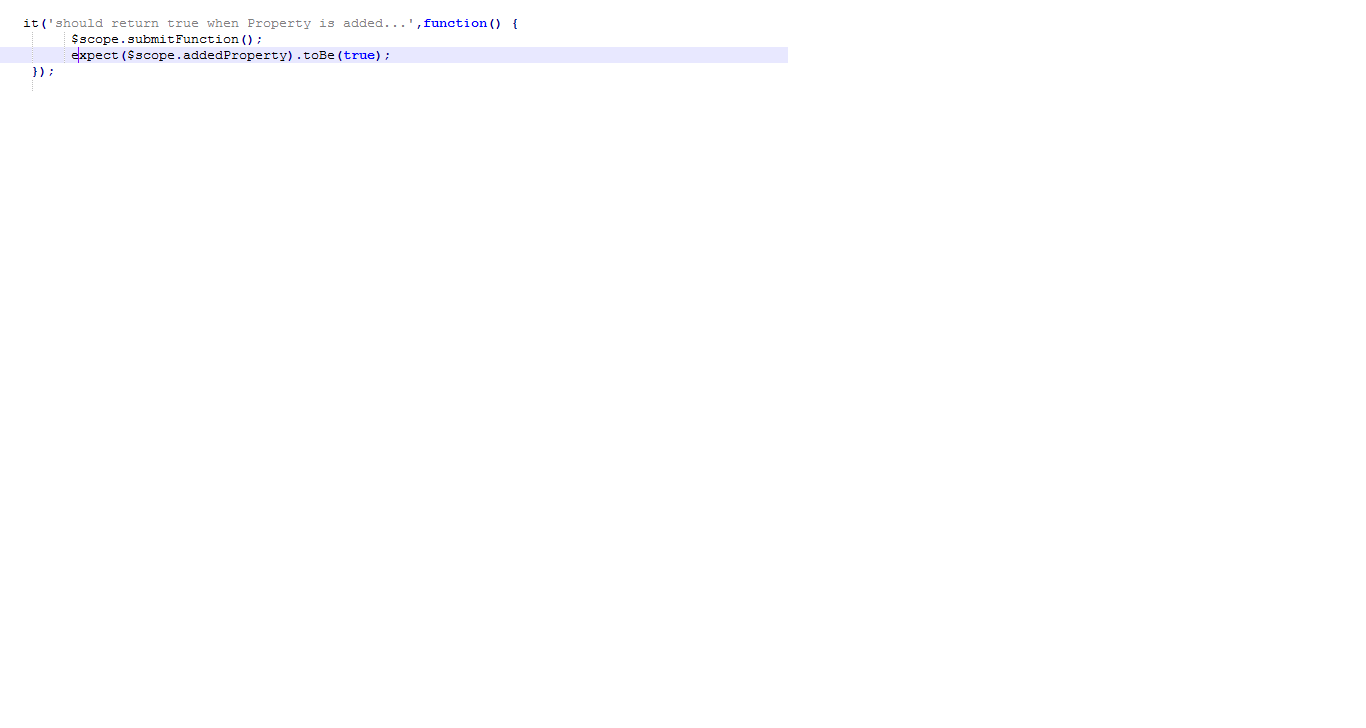
\includegraphics[width=1\textwidth]{./Images/input6.png}

\paragraph{Outcome: } The function will throw a NullPointerException


\section{Item Pass/Fail Criteria}
Each item tested must meet a certain criteria in order to pass. These criteria are as follows:\\

AddPropertyValidation
\begin{itemize}
 \item the property must not exist in the database
 \item the input in the parameters must be invalid
\end{itemize}
DeletepropertyValidation
\begin{itemize}
 \item the property must not exist in the database
 \item the input in the parameters must be invalid
\end{itemize}
FindProperty
\begin{itemize}
 \item the back end server must be running
 \item the property must not exist in the database
 \item the input in the parameters must be valid
\end{itemize}
Test the encoded String 
\begin{itemize}
 \item the must values in the string
\end{itemize}
Add Property front-end 
\begin{itemize}
 \item The must values in the string
 \item session ID must be initialised
\end{itemize}
Retrieve a property
\begin{itemize}
 \item the back end server must be running
 \item the property must not exist in the database
 \item the input in the parameters must be valid
\end{itemize}
\section{Test Deliverables}
Artefacts to be produced as part of unit testing include the following:
\begin{itemize}
\item Test Plan
\item Test Report
\item Link to Test Code
\end{itemize}

%Unit test Report page
\newpage
\begin{center}
{\huge \bfseries Unit Test Report}\\[0.5cm]
\end{center}
\section{Detailed Test Results}
\subsection{Overview of Test Results}
The test that were done were mostly on the back-end.This is where we validate our values before they are inserted into the database.all the test we did passed even those that would cause the systems fail. This was done by handling the system failure correctly,anticipating what would go wrong and handling that failure in a correct way through try and catch blocks. Junit spring framework was used for unit testing in the back-end. The front-end test where done to the test the system in a wider scope because the front-end is depended on the back-end.when a test that sends a request to the back-end passes, it also assures that the function in the back-end are working correctly.We used Karma and Jasmine framework to conduct unit test in javascript.

\subsection{Functional Requirements Test Results}
The tests we have created for this module are contained within the file   \href{https://github.com/u13278012/IMPAKD/blob/master/Implementation/PIO/BackEnd/test/Test/PropertyTest.java}{PropertyTest}, \href{https://github.com/u13278012/IMPAKD/blob/master/Implementation/PIO/FrontEnd/app/addProperty/addProperty_test.js}{Font-End Test} and \href{https://github.com/u13278012/IMPAKD/}{gitHub}.

\subsubsection{Test Case 1 (TC 4.1)}
The correct information was passed to the \$http request
\paragraph{Result: Pass.}

\subsubsection{Test Case 2 (TC 4.2)}
The property list was returned and the name was extracted
\paragraph{Result: Pass.}

\subsubsection{Test Case 3 (TC 4.3)}
The invalid value was handled though a try and catch block by throwing an ArithmeticException 

\paragraph{Result: Pass.}
\subsubsection{Test Case 4 (TC 4.4)}
The invalid value was handled though a try and catch block by throwing an ArithmeticException 

\paragraph{Result: Pass.}

\subsubsection{Test Case 5 (TC 4.5)}
The invalid value was handled though a try and catch block 
\paragraph{Result: Pass.}

\subsubsection{Test Case 6 (TC 4.6)}
The function returned true, hence it successfully persisted in the database
\paragraph{Result: Pass.}
\section{Other}
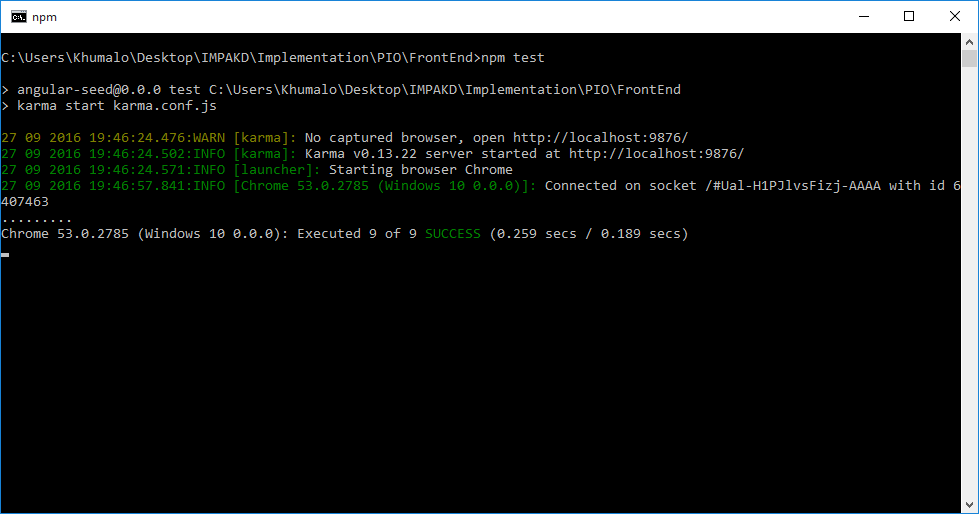
\includegraphics[width=1\textwidth]{./Images/AddPropertyKarmaTest.png}\\
Front-End Test results \\

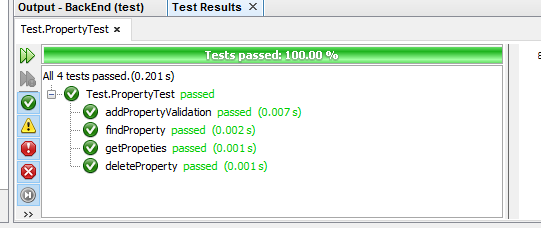
\includegraphics[width=1\textwidth]{./Images/testResults.png}\\
Back-End Test results \\


\section{Conclusions and Recommendations}
Test were done on the back-end to test for security features implemented as the application allows users to input data.Parameters are passed though the url to the back-end. So regardless of the validation we have in the font-end, malicious users might pass in  malicious code after the validation in the front-end through the url, so it is important for the application to handle both user errors and malicious code, the test have assured that the countermeasures implemented work correctly.

\end{document}

